\section{Эксперименты}\label{sec:exps}

\paragraph{Бейслайн.} Здесь мы приводим основные сведения о моделях и алгоритмах, с которыми мы сравниваем нашу.

1) Мы оцениваем эффективность описанного фреймворка (раздел \ref{sec: framework}), в частности, Sparse-, Contrastive-, $\ell_1$-CBMs, сравнивая его с предыдущими Label-free \cite{oikarinen2023labelfree}, Post-hoc CBM \cite{yuksekgonul2023posthoc}, LaBo \cite{yang2023language} фреймворки на одних и тех же наборах данных \cite{5206848,wah_branson_welinder_perona_belongie_2011,krizhevsky2009learning,7968387}, но с разными базовыми моделями: в то время как в экспериментах с фреймворком Label-free, проведенных с ResNet50 \cite{he2015deep} и CLIP(ResNet50)\cite{radford2021learning}, мы используем только варианты архитектуры CLIP в качестве основы. Заметим, что оба фреймворка получают довольно схожие концепции, поскольку Label-free также включает опцию генерации концепций с помощью ConceptNet API. Также модель Label-free обучается двумя алгоритмами последовательно: сначала обучается CBLs с cos-cubed сходством, введенным в \cite{oikarinen2023labelfree}, затем последний FC-слой обучается с помощью решателя GLM-SAGA \cite{pmlr-v139-wong21b}. Мы также приводим сравнение с линейным зондированием, когда один линейный слой после CLIP обучается классификации. Подробное объяснение эксперимента с зондированием мы приводим в \cref{sec:appendix}.

2) Мы оцениваем эффективность описанного алгоритма Concept Matrix Search (раздел \ref{sec:cms}), сравнивая его с предыдущей работой Visual Classification via Description, которую мы обозначаем как метод "DescriptionCLS" в \cref{tab:cbms_tab}. Оба метода схожи в том, что они способны различать классы, выбирая тот, который имеет наивысший балл, предоставляемый некоторым \textit{rule}, и оба они не обучают никакую модель и используют только эмпирические формулы для предсказания целей более интерпретируемым способом. Наш \textit{rule} - это CMS (см. \cref{Alg:CMS}), в то время как метод "DescriptionCLS" опирается на функцию, которая дает оценку классу на основе того, сколько концептов этого класса чувствительны к изображению этого самого класса. Чувствительность понятия измеряется как логарифмическая вероятность того, что понятие относится к изображению в соответствии с косинусным сходством. CMS также использует эту меру, но она не создает прямого отображения класс-концепт, вместо этого мы проводим классификацию в более общем виде, учитывая только партию изображений и все концепции с классами. Кроме того, Concept Matrix Search играет роль более общего классификатора, и мы сравним их ниже, что весьма информативно, поскольку оба метода используют одну и ту же модель CLIP в качестве основы. Кроме того, необходимо привести сравнение с классификацией изображений с нулевым снимком. В этом случае мы рассматриваем пакет изображений и названия классов как входные данные для кодирования CLIP, который, в свою очередь, выдает матрицу "изображение - класс". Выполнив операцию argmax, мы определяем наиболее близкий класс.

\setcounter{table}{1}
\begin{table*}[t]
\caption{Сравнение перформанса Bottleneck моделей на основных датасетах. Мы наблюдаем превосходство Sparse-CBM над другими архитектурами на CIFAR10, CIFAR100 и CUB200 датасетах.}
\label{tab:cbms_tab}
\begin{center}
\begin{small}
\begin{sc}
\begin{tabular}{lccccr}
\toprule
Model & CIFAR10 & CIFAR100 & ImageNet & CUB200 & Places365 \\
\midrule
Sparse-CBM (Ours)    & \textbf{91.17\%} & \textbf{74.88\%} & 71.61\% & \textbf{80.02\%} & 41.34\% \\
$\ell_1$-CBM (Ours) & 85.11\% & 73.24\% & 71.02\% & 74.91\% & 40.87\%\\
Contrastive-CBM (Ours)   & 84.75\% & 68.46\% & 70.22\% & 67.04\% & 40.22\% \\
Label-free CBM    & 86.40\% & 65.13\% & \textbf{71.95\%} & 74.31\% & \textbf{43.68\%}    \\
Post-hoc CBM (CLIP)   &  83.34\%       &   57.20\%      &     62.57\%         &   63.92\%      &       39.66\%        \\
LaBo (full-supervised)             & 87.90\%&       69.10\%    &    70.40\%     & 71.80\% & 39.43\%
\\
\hline
Linear Probing             & 96.12\%&       80.03\%     &    83.90\%     & 79.29\% & 48.33\%     \\
\bottomrule
\end{tabular}
\end{sc}
\end{small}
\end{center}
\end{table*}
\begin{table*}[t]
\caption{Сравнение CMS и "DescriptionCLS"  на основных датасетах.}
\label{tab:cms_tab}
\begin{center}
\begin{small}
\begin{sc}
\begin{tabular}{lccccr}
\toprule
Method & CIFAR10 & CIFAR100 & ImageNet & CUB200 & Places365 \\
\midrule
CMS (Ours)    & \textbf{85.03\%} & 62.95\% & \textbf{77.82\%} & \textbf{65.17\%} & 39.43\% \\
DescriptionCLS  &    81.61\%     &      \textbf{68.32\%}    &     75.00\%     &   63.46\%    &   40.55\%    \\
Zero-shot  &    81.79\%     &      52.84\%    &     76.20\%     &   62.63\%    &   \textbf{41.12\%}    \\
\bottomrule
\end{tabular}
\end{sc}
\end{small}
\end{center}
\end{table*}

\subsection{CBM эксперименты}
\label{sec:cbmexp}

\paragraph{Набор концептов.} Мы сгенерировали большие наборы: один с 6 500 концептами, используя Llama-2, и второй с 5 000 концептами, используя ConceptNet \cite{article} API, и обработали их с помощью трансформатора предложений 'all-mpnet-base-v2', чтобы найти отсечения сходства, упомянутые в \textbf{шаг 2} (см. \cref{sec:framework}). API и обработали их с помощью трансформатора предложений 'all-mpnet-base-v2', чтобы найти отсечки сходства, упомянутые в \textbf{Шаг 2} (см. \cref{sec:framework}). Для самого большого набора мы подготовили все метки классов, чтобы создать из них концепты. Более того, для каждого набора данных в \cref{tab:concepts_size} также представлен соответствующий набор концептов. Мы называем самый большой набор концептов "Все концепты", который можно увидеть в \cref{fig:cms_acc}. Каждый набор данных имеет свой собственный набор концептов, сгенерированный из классов набора данных в соответствии с \textbf{шаг 2}. Для корректного сравнения, представленные в \cref{tab:cbms_tab} модели были обучены \textit{only} с концептами, сгенерированными ConceptNet.

\paragraph{Модели.} CLIP-ViT-L/14 и B/32\footnote{Упомянутую модель CLIP-ViT-B/32 можно найти на хабе Hugging Face \texttt{https://huggingface.co/openai/clip-vit-base-patch32}} в качестве основы для всех CBM-экспериментов. В зависимости от набора данных, размер этих моделей варьируется. Самая маленькая конфигурация B/32
\begin{figure}%{0.285\textwidth}
\setcounter{table}{0}
\captionof{table}{Зависимость размера набора концептов от набора данных.}
\label{tab:concepts_size}
\begin{center}
\begin{small}
\begin{sc}
\begin{tabular}{lr}
\toprule
 Dataset & \# of concepts   \\
\midrule
CIFAR10  & 120   \\
CIFAR100 & 944 \\
ImageNet & 4,751 \\
CUB200 & 926 \\
Places365 & 2,900\\
"All concepts" & 5,051 \\
\bottomrule
\end{tabular}
\end{sc}
\end{small}
\end{center}
\end{figure}
 для CIFAR10 имеет размер 151,3 млн параметров и 50 000 обучаемых параметров, что эквивалентно 0,6 ГБ. Самая большая - L/14 для ImageNet-1K: 455 миллионов параметров; 27,3 миллиона обучаемых параметров и размер 1,81 ГБ. Для наглядности мы показываем точную информацию в \cref{tab:backbone_nets} (до обучения). А в \cref{tab:cbms_tab} мы приводим результаты для конфигурации CLIP-ViT-L/14.

\paragraph{Оборудование.}
Мы обучали наши модели на одной машине с 4 графическими процессорами NVIDIA A100-SXM4-80GB и A100-PCIE-40GB, по два каждого типа. Для наших конфигураций МД каждый шаг обучения со скоростью обучения по умолчанию, указанной в таблицах \ref{tab:backbone_nets}, \ref{tab:concepts_size} данных, занял менее 1 секунды для конфигурации CLIP-ViT-B/32 backbone и немного больше для CLIP-ViT-L/14. Мы обучили каждую из моделей Sparse, $\ell_1$, Contrastive-CBM на ImageNet-1K \cite{russakovsky2015imagenet} за 20 000 шагов, что заняло чуть больше 5,5 часов для каждой модели (см. \cref{fig:curves}). Наши реализации не зависят от конкретных аппаратных архитектур.

\begin{figure}[t]
\begin{center}
\centerline{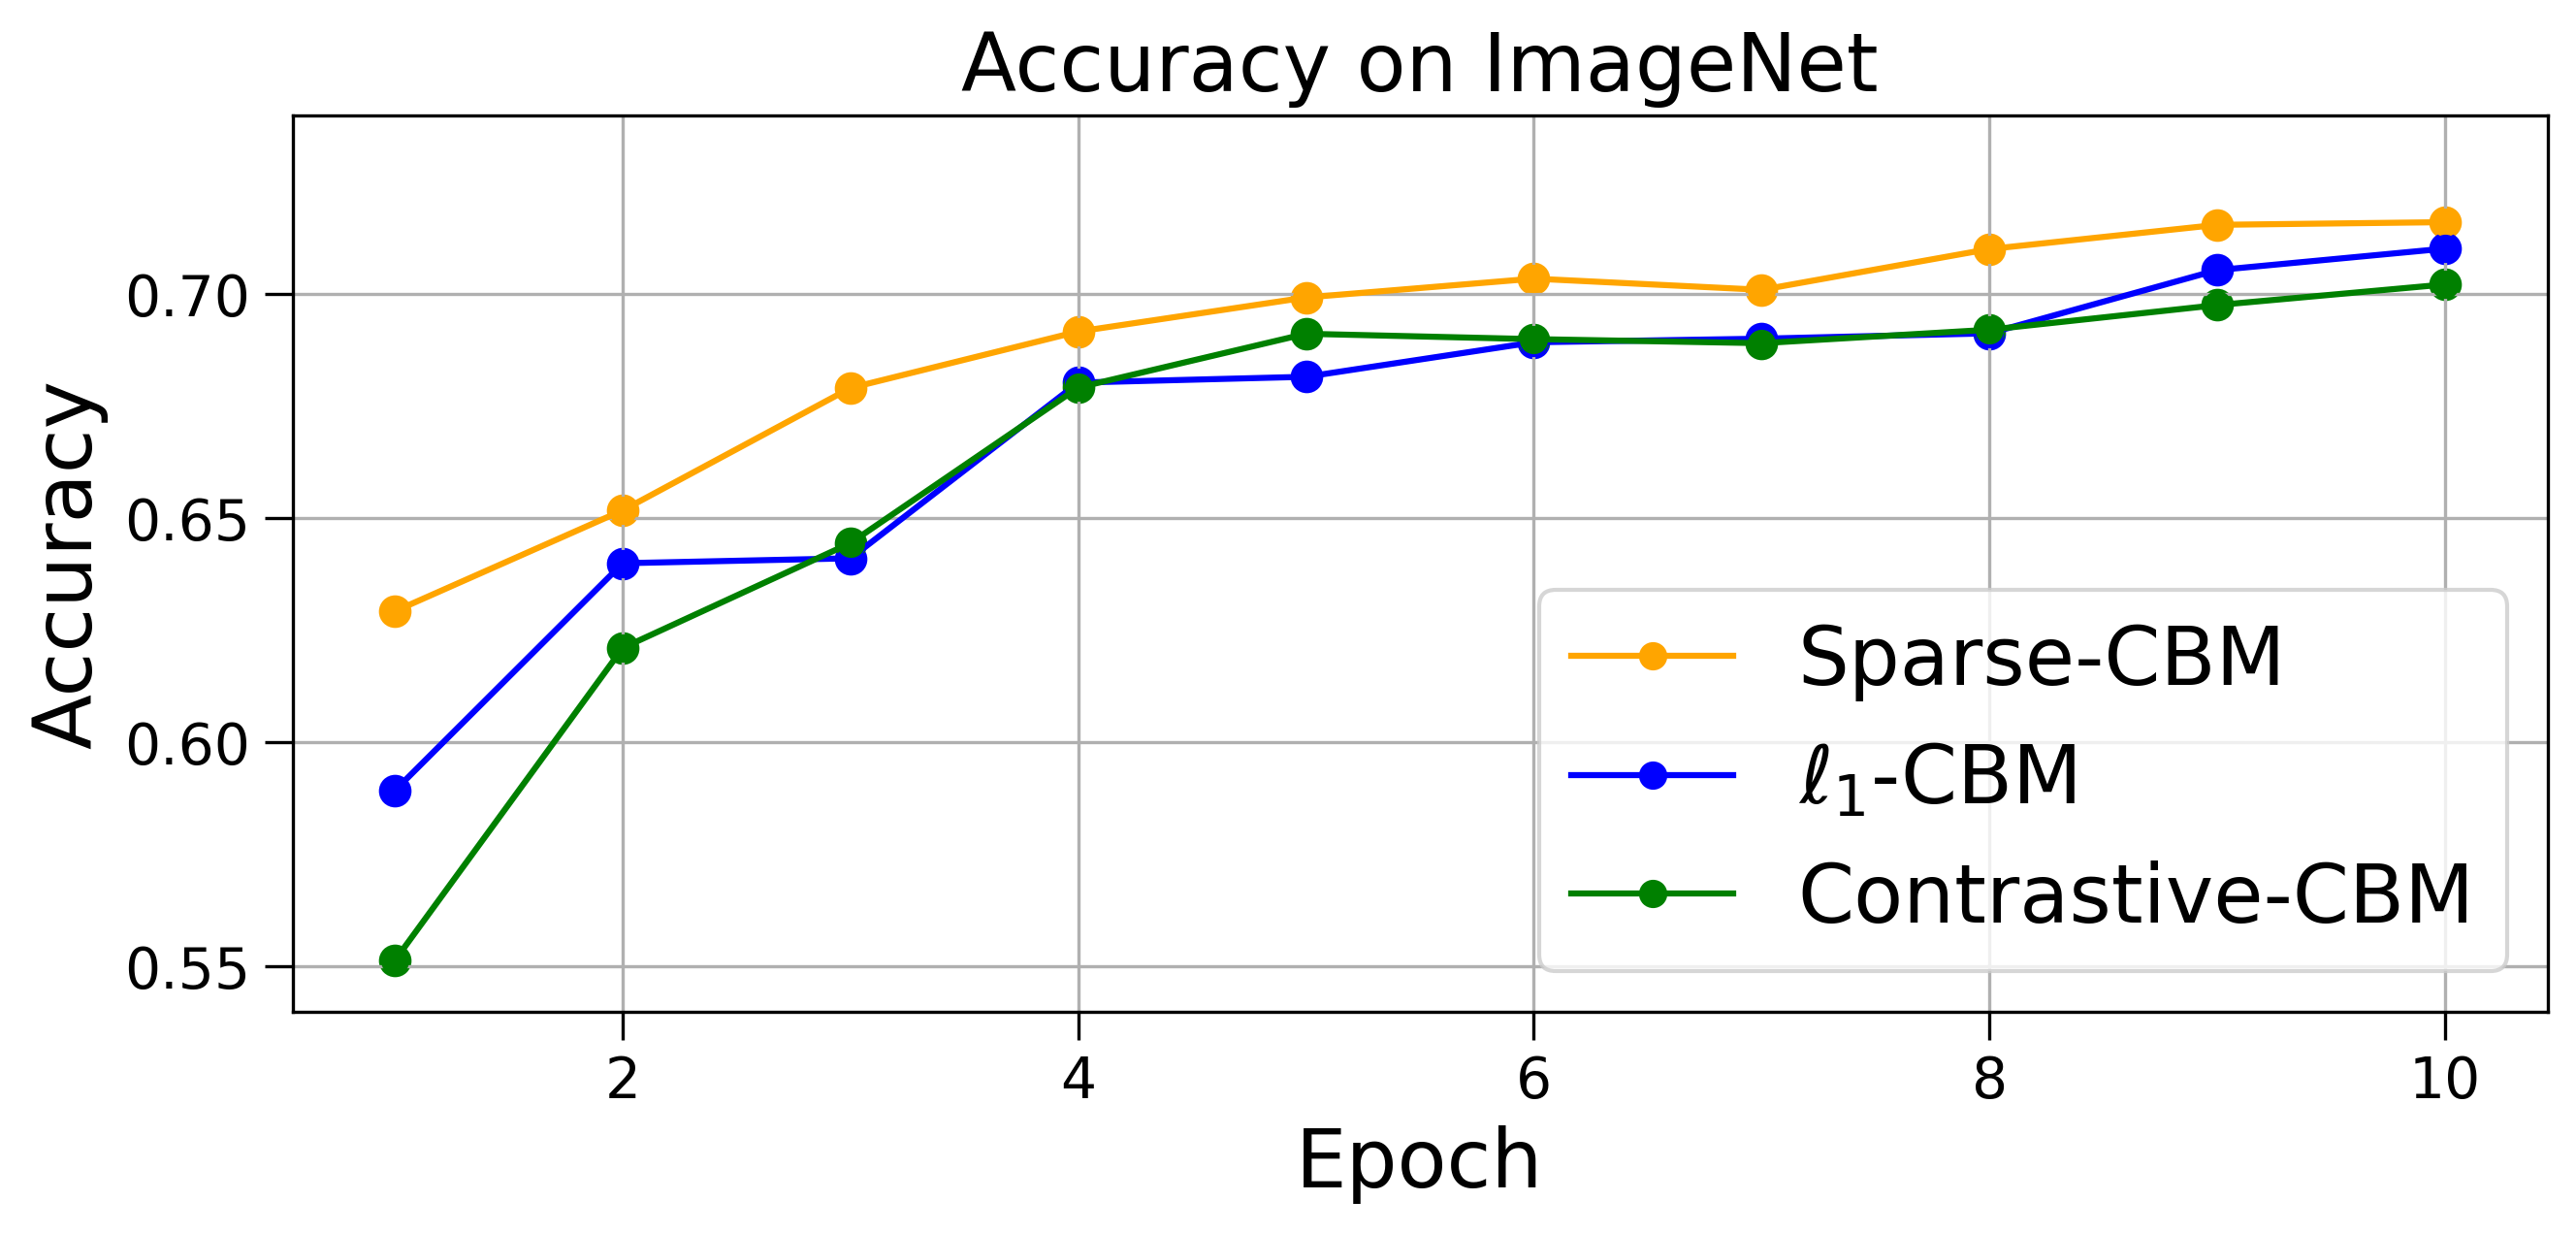
\includegraphics[width=\columnwidth]{./figures/cbms_acc_imnet.png}}
\caption{Сравнение CBM мотодов на валидационной подвыборке датасета ImageNet.}
\label{fig:cbm_acc}
\end{center}
\vskip -0.45in
\end{figure}
\paragraph{Рабочая нагрузка}. Мы поддерживаем схему \textit{последовательных узких мест} из \cite{koh2020concept}. Действительно, сначала мы производим градиентное обновление весов $W_{\mathrm{F}}$ и $W_{\mathrm{CBL}}$ с учетом их параметров независимо друг от друга, а затем, во время следующего прохода вперед, FC получает на вход логиты из обновленного CBL. Таким образом, после каждой итерации задач минимизации CBL и FC для классификатора создается новое представление концепта.

\subsection{CMS эксперименты}
\label{sec:cmsexp}

В этом разделе мы сравним два алгоритма: наш CMS \ref{Alg:CMS} и основной метод, предложенный в \cite{menon2022visual}. Оба они используют базовые возможности модели CLIP. Мы тестируем их на одной и той же конфигурации CLIP-ViT-L/14. Мы показали превосходство нашего метода на нескольких наборах данных, которые можно увидеть в \cref{tab:cms_tab}. Авторы \cite{kazmierczak2023clipqda} измерили зависимость точности при обнулении определенного количества концептов, а \cite{chauhan2023interactive} исследовали влияние нескольких относительных концептов. Мы же измерили зависимость точности от различных наборов понятий: почти синонимов (сходство "понятие-класс" 0,95 вместо 0,85), сгенерированных ConceptNet как обычно, одного набора многих понятий (большинство из них бесполезны для данных CIFAR10) и 3 000 случайно сгенерированных слов. Результаты представлены в \cref{fig:cms_acc}.